\documentclass[12pt,a4paper]{article}
\usepackage[left=2cm,top=2cm,right=2cm,bottom=2cm,head=.5cm,foot=.5cm]{geometry}

\usepackage[sc]{titlesec}
\usepackage{graphicx}
\usepackage{xcolor}
\usepackage[many]{tcolorbox}

\usepackage[utf8]{inputenc}
\usepackage[english]{babel}
\usepackage[english]{isodate}
\usepackage[parfill]{parskip}
\usepackage[hidelinks]{hyperref}
\hypersetup{
colorlinks=true,
linkcolor=black,
citecolor=black,
anchorcolor=black,
filecolor=black,
menucolor=black,
runcolor=black,
urlcolor=orange
}

\definecolor{canary}{RGB}{255,255,153}

\newtcolorbox{myboxii}[1][]{
  breakable,
  freelance,
  title=#1,
  colback=canary,
  colbacktitle=canary,
  coltitle=black,
  fonttitle=\bfseries,
  bottomrule=0pt,
  boxrule=0pt,
  colframe=white,
  overlay unbroken and first={
  \draw[red!75!black,line width=3pt]
    ([xshift=5pt]frame.north west) -- 
    (frame.north west) -- 
    (frame.south west);
  \draw[red!75!black,line width=3pt]
    ([xshift=-5pt]frame.north east) -- 
    (frame.north east) -- 
    (frame.south east);
  },
  overlay unbroken app={
  \draw[red!75!black,line width=3pt,line cap=rect]
    (frame.south west) -- 
    ([xshift=5pt]frame.south west);
  \draw[red!75!black,line width=3pt,line cap=rect]
    (frame.south east) -- 
    ([xshift=-5pt]frame.south east);
  },
  overlay middle and last={
  \draw[red!75!black,line width=3pt]
    (frame.north west) -- 
    (frame.south west);
  \draw[red!75!black,line width=3pt]
    (frame.north east) -- 
    (frame.south east);
  },
  overlay last app={
  \draw[red!75!black,line width=3pt,line cap=rect]
    (frame.south west) --
    ([xshift=5pt]frame.south west);
  \draw[red!75!black,line width=3pt,line cap=rect]
    (frame.south east) --
    ([xshift=-5pt]frame.south east);
  },
}

\usepackage{url}

\usepackage{listings}
\lstset{%
basicstyle=\small\ttfamily,
backgroundcolor=\color{green!5}, % light blue background
showspaces=false,
showstringspaces=false,
showtabs=false,
numbers=left,
numbersep=5pt,
numberstyle=\footnotesize\ttfamily,
frame=single,
breaklines=true,
breakatwhitespace=false} % orange strings

\usepackage{fancyhdr}
\pagestyle{fancy}
\lhead{}
\rhead{\nouppercase\leftmark}

\usepackage{textcomp}
\usepackage{upquote}

\usepackage{fontspec}

\begin{document}
\setmainfont{GFS Didot}

\vspace*{\fill}

\thispagestyle{empty}

\begin{center}

\begin{figure}[!htbp]
    \centering
	
\includegraphics[width=\textwidth]{../src/images/splash.png}
\end{figure}

\vspace{1cm}

\textsc{\Huge{Documentation}}

\vspace{3cm}

\Large{Version 1.001\\}
\today

\vspace{3cm}

\url{https://dgkontopoulos.github.io/Structuprint/}

\end{center}

\vspace*{\fill}
\newpage

\vspace*{\fill}
\vspace{-5cm}
\tableofcontents
\vspace*{\fill}
\newpage

\section{Introduction}
Structuprint is a software tool for two-dimensional visualisation of surfaces 
of PDB structures. Details about the algorithm executed by Structuprint will be 
soon made available, in the form of a scientific publication. 
The name stems from the fingerprint-like figures that it 
produces (see below); one could think of them as the fingerprints of protein 
structures. As this name can be used both for the tool itself and its 
resulting figures, from now on \underline{\textbf{S}}tructuprint 
(with an uppercase "S") will refer to the software, whereas 
\underline{\textbf{s}}tructuprint (with a lowercase "s") to the figure 
generated with it.\\

This is how a structuprint looks like:
\begin{figure}[!htbp]
    \centering
	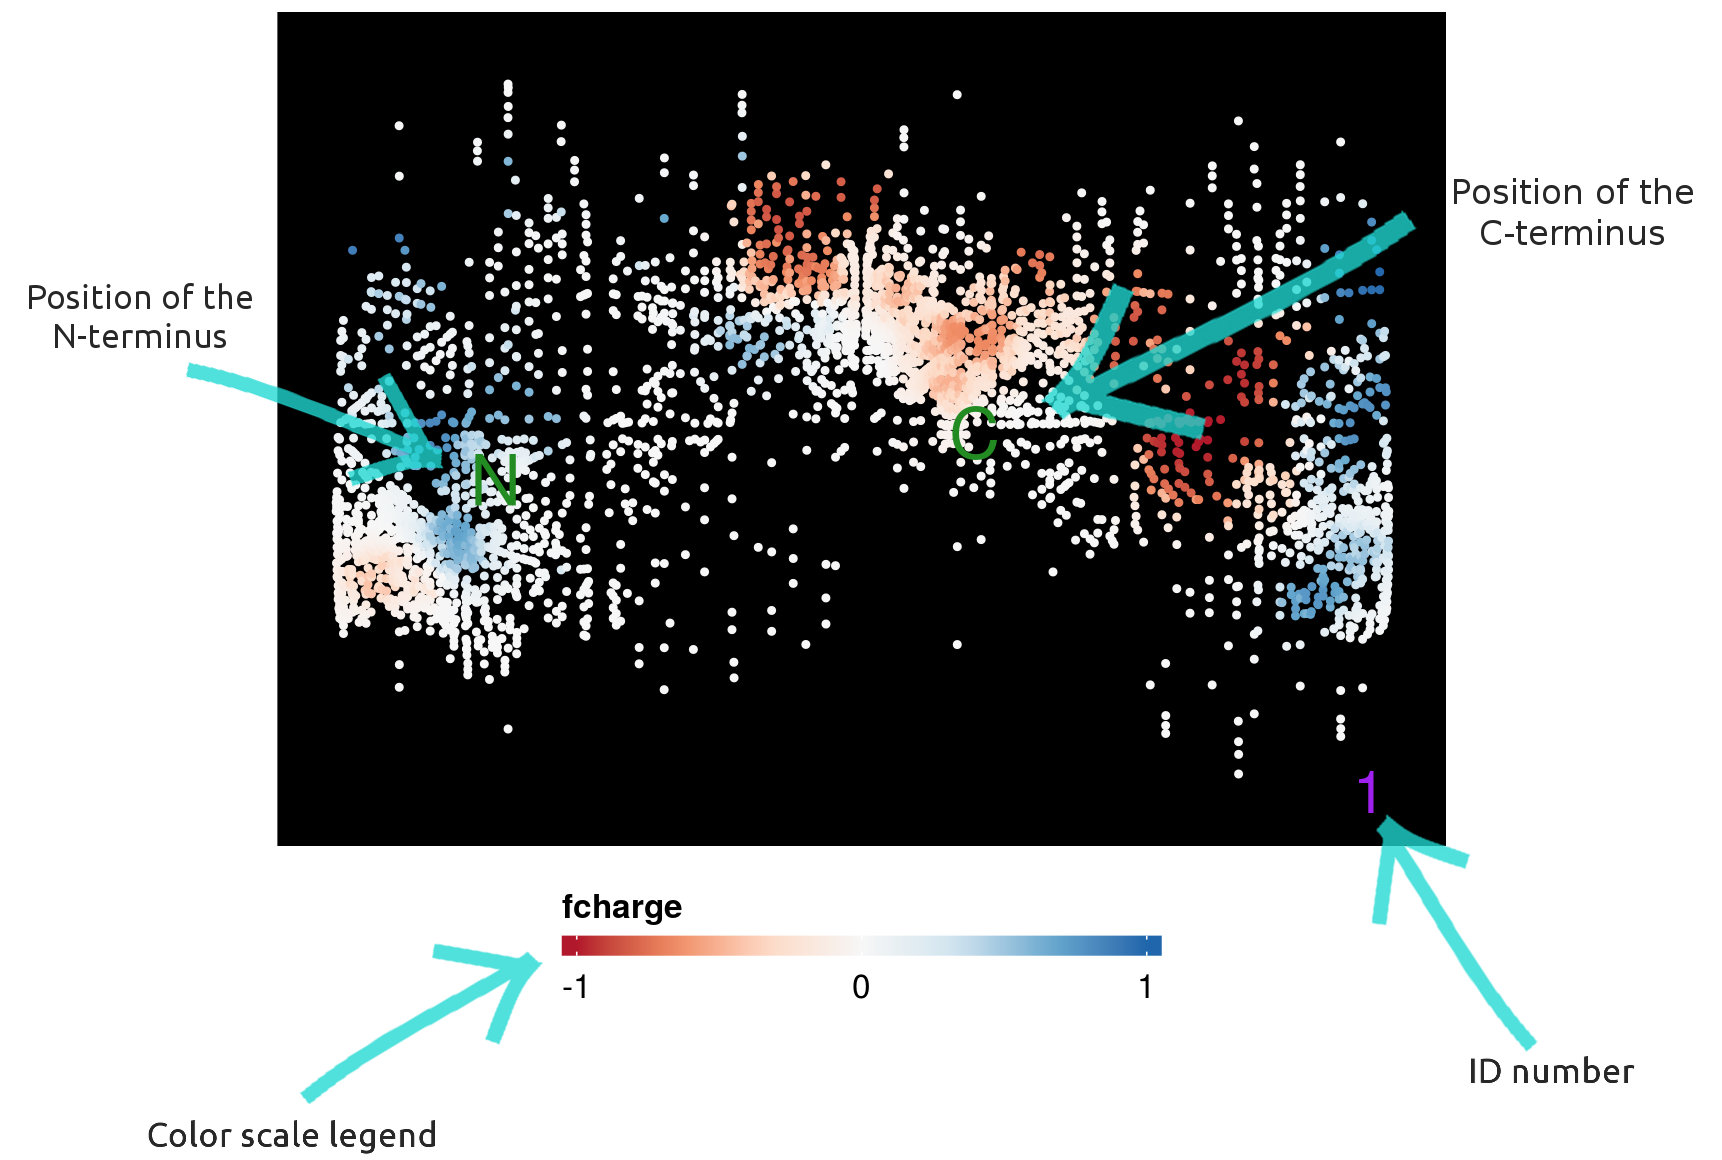
\includegraphics[width=\textwidth]{figures/structuprint.png}
\end{figure}

\vspace{-0.5cm}

The data points in the figure are colored according to the value of a selected 
property, in this case \path{fcharge}, i.e. charge. In total, the values of 328 
physico-chemical properties have been pre-calculated for the 20 common amino acids using 
\href{http://www.chemcomp.com/MOE-Molecular_Operating_Environment.htm}
{MOE 2012.10}. See the amino acid properties 
codebook for a list of the available properties and their explanations. 
At the bottom of the figure lies the color scale legend, along with its title 
which can be set by the user.\\

The green N and C letters show the approximate positions of the N- and C-termini. 
Structuprint treats each model in the PDB file as a 
different polypeptide chain, so the N- and C-termini correspond to the first 
and last residue in the model.\\

The purple number at the bottom right corner indicates the ID number of the PDB file. All 
of these features are optional and can be disabled.

Apart from a single figure like the one shown above, Structuprint can 
also produce animations from multiple PDB files. Therefore, to allocate 
the execution of different tasks, the tool consists of three 
scripts: i) \path{structuprint}, ii) \path{structuprint_frame} 
and iii) \path{structuprint_gui}.\\
\newline
The core algorithm that transforms a 3D PDB file into a 2D figure is 
executed by \path{structuprint_frame}. For animations, 
\path{structuprint} coordinates the generation of multiple frames 
and joins them into a GIF file at the end. Finally, \path{structuprint_gui} 
provides a Graphical User Interface to the above tasks. The figure 
below shows the relationships among the 3 scripts.
\begin{figure}[!htbp]
    \centering
	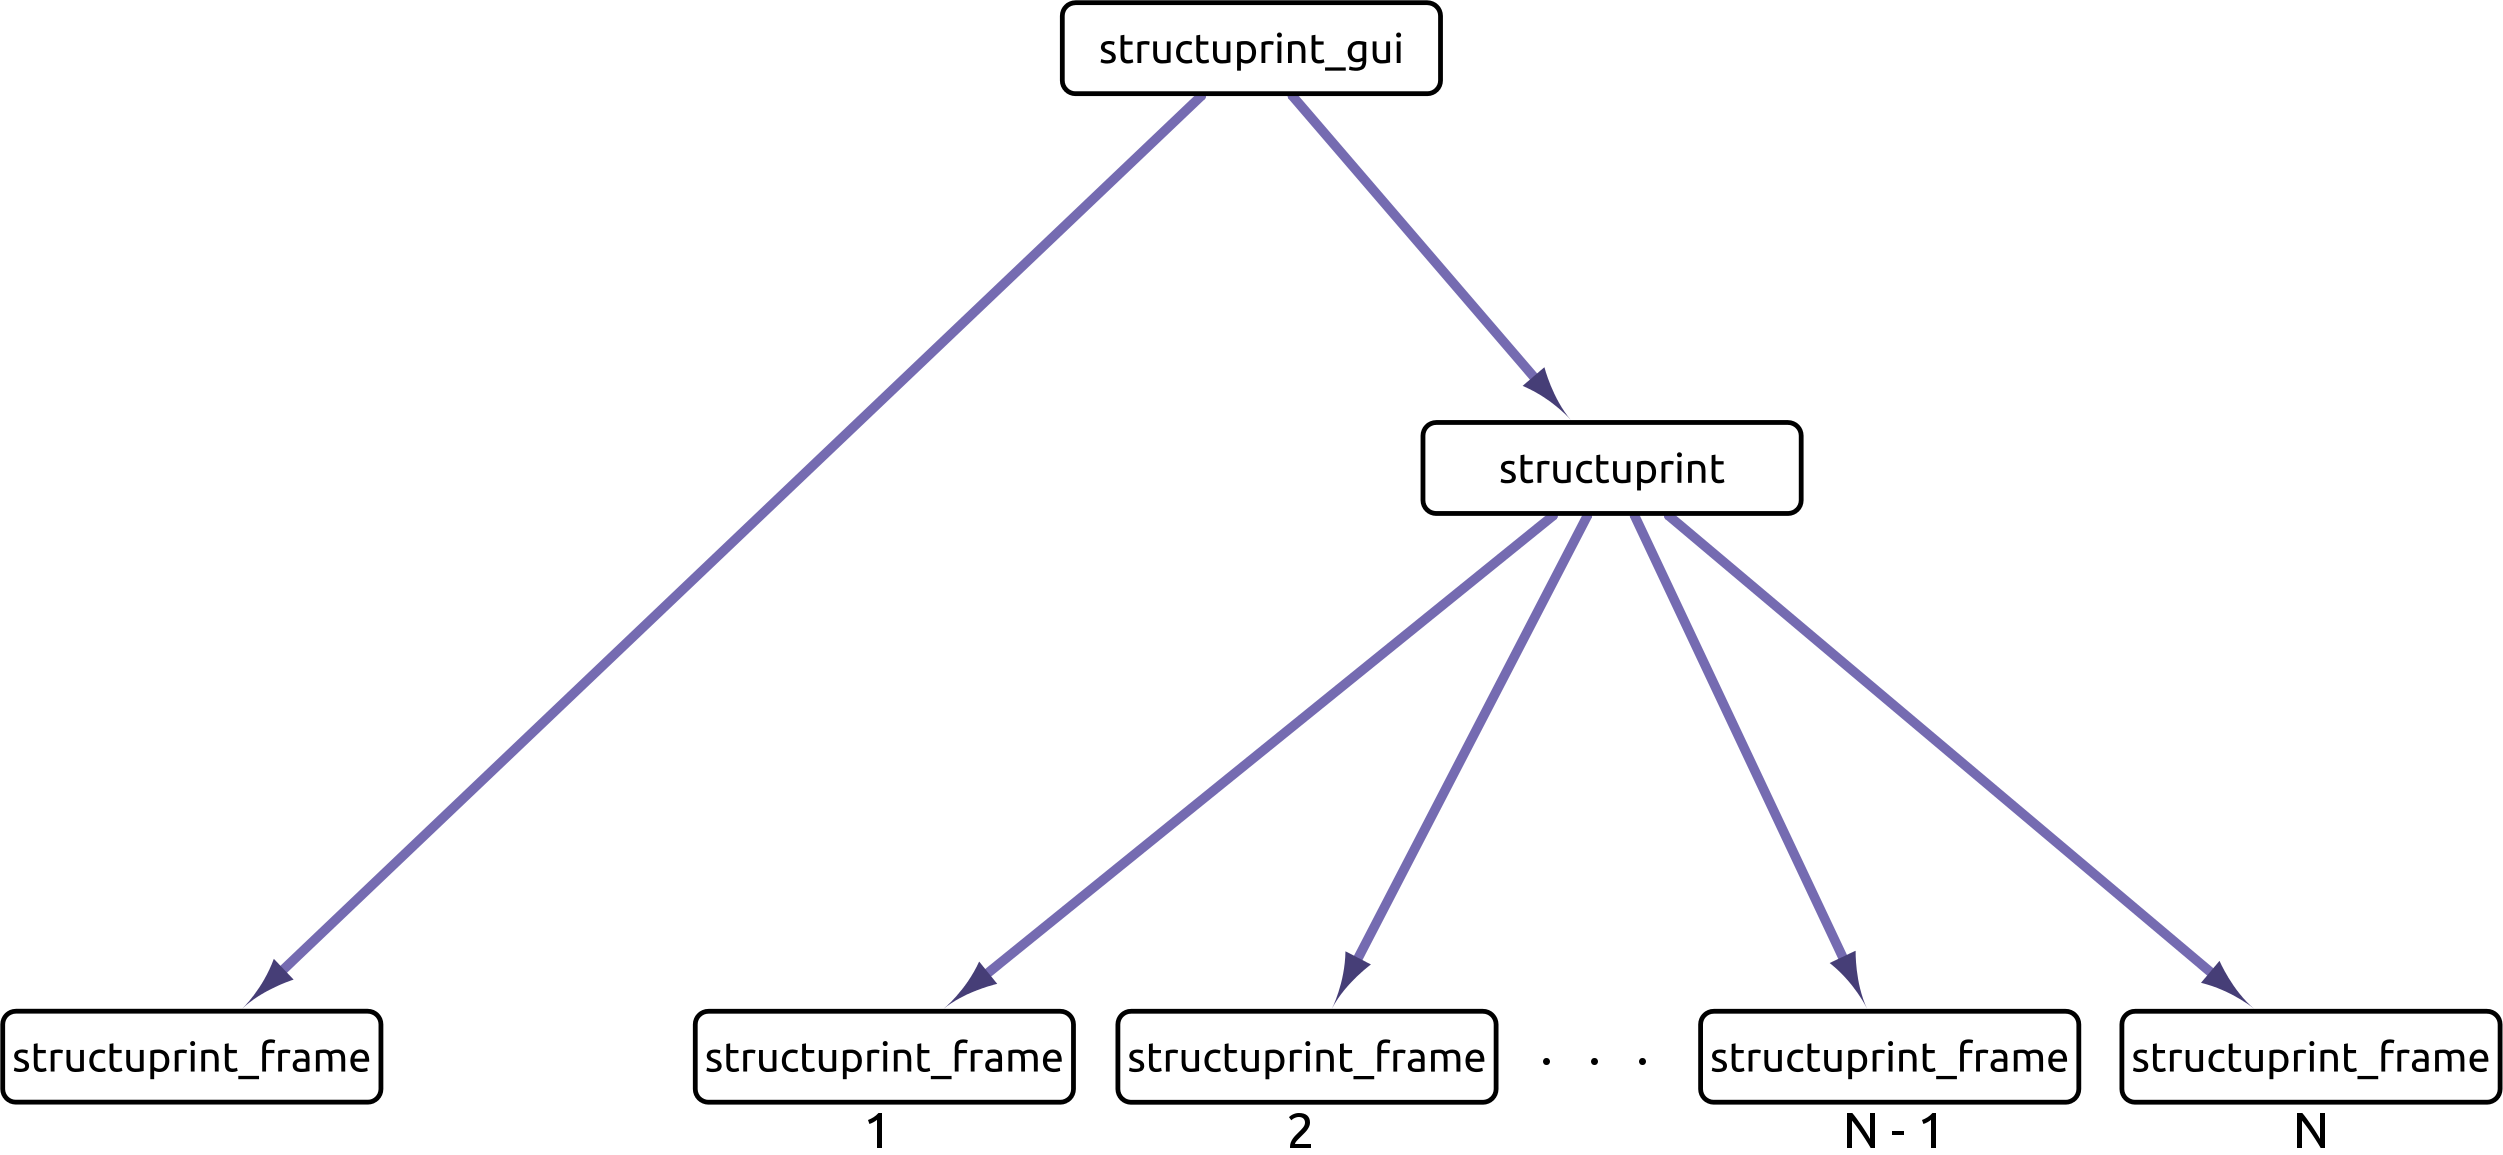
\includegraphics[width=\textwidth]{figures/diagram.png}
\end{figure}

The \path{structuprint} script expects PDB filenames to contain 
an underscore and an ID number before the '.pdb' suffix (e.g. mds\_1.pdb). 
The input directory can contain multiple numbered PDB files. Instead, 
\path{structuprint_frame} requires that the input directory contains only 
a single PDB file that may or may not be numbered.

\newpage

\section{Installing Structuprint}
\subsection{From prebuilt packages}
Prebuilt packages and installers are available from Structuprint's website. 
They handle the installation of the program along with any needed 
dependencies. An exception is the package for CentOS Linux, which requires  
that the \path{epel-release} package is already installed, before the Structuprint 
package can be used.

\subsection{From the source code (un*x systems only)}
The source code is available from Structuprint's GitHub repository at 
\url{https://github.com/dgkontopoulos/Structuprint}. Download the 
latest release as a compressed file and uncompress it:
\begin{lstlisting}[numbers=none]
tar xzvf structuprint_src_1_00.tar.gz && cd structuprint_1_00/
\end{lstlisting}

A \path{structuprint_1_00} directory will be created. Inside it, you 
will find a \path{Makefile}. While inside that directory, type the 
following commands:
\begin{lstlisting}
make test
make
make install
\end{lstlisting}
Line 1 will run some tests to make sure that all dependencies are available. 
When installing Structuprint from the source code, you have to install all 
required dependencies manually. These comprise the \path{perl} and \path{R} 
executables, but also Perl modules (\path{Astro::MapProjection}, 
\path{Bio::PDB::Structure::Atom}, \path{DBI} ...) and R packages 
(\path{ggplot2}, \path{grid}, \path{scales}, \path{labeling}). Some of them have 
their own dependencies, but you may be able to install them all at once 
via your package manager (e.g., \path{apt-get} on Debian or \path{pacman} 
on Arch Linux).\\

\begin{myboxii}[\begin{center}Useful installation tutorials\end{center}]
\begin{tabular}{ll}
-Perl modules: & \url{http://perlmaven.com/how-to-install-a-perl-module-from-cpan}\\
-R packages: & \url{http://www.r-bloggers.com/installing-r-packages/}
\end{tabular}
\end{myboxii}

\vspace{0.5cm}

Line 2 will make the scripts executable and line 3 will install all the 
necessary files at \path{/opt/structuprint/}. To change the installation 
directory, type:
\begin{lstlisting}[numbers=none]
make install -PREFIX=/PATH/TO/CUSTOM/DIR
\end{lstlisting}

To uninstall Structuprint, type the following command, followed by a 
\path{PREFIX} argument, if needed:
\begin{lstlisting}[numbers=none]
make uninstall
\end{lstlisting}

\newpage

\section{\texttt{structuprint}'s manpage}
\textbf{\large{NAME}}

\path{structuprint} - utility for 2D animations of protein surfaces\\

\textbf{\large{SYNOPSIS}}

\texttt{\textbf{structuprint} \textbf{-prop} PROPERTY\newline
\hspace*{2.66cm} \textbf{-dir} INPUT\_DIRECTORY\newline
\hspace*{2.66cm} [\textbf{-outdir} OUTPUT\_DIRECTORY]\newline
\hspace*{2.66cm} [\textbf{-custom\_db} PATH\_TO\_DATABASE]\newline
\hspace*{2.66cm} [\textbf{-height} HEIGHT] [\textbf{-width} WIDTH]\newline
\hspace*{2.66cm} [\textbf{-res} PPI\_NUMBER]\newline
\hspace*{2.66cm} [\textbf{-point\_size} SIZE]\newline
\hspace*{2.66cm} [\textbf{-bgcol} HEX\_COLOR$|$COLOR\_NAME] [\textbf{-bgalpha} ALPHA\_VALUE]\newline
\hspace*{2.66cm} [\textbf{-legend\_title} TITLE]\newline
\hspace*{2.66cm} [\textbf{-{}-no\_ID}] [\textbf{-{}-no\_legend}] [\textbf{-{}-no\_NC}]\newline
\hspace*{2.66cm} [\textbf{-{}-del\_temp\_dirs}]\newline
\hspace*{2.66cm} [\textbf{-delay} DELAY]\newline
\hspace*{2.66cm} [\textbf{-nloops} NUMBER\_OF\_LOOPS]\newline
\hspace*{2.66cm} [\textbf{-nthreads} NUMBER\_OF\_THREADS]\newline
\hspace*{2.66cm} [\textbf{-{}-help}]\\
\hspace*{2.66cm} [\textbf{-{}-properties}]}\\

\textbf{\large{DESCRIPTION}}

\path{structuprint} is a tool for generating two-dimensional animations of 
protein surfaces. Given an input directory with properly named PDB files, 
\path{structuprint} will render each frame separately and join them into an animation 
at the end.\\

\textbf{\large{OPTIONS}}
\begin{description}

\item[{\textbf{-bgalpha} ALPHA\_VALUE}] \mbox{}

Set the transparency level of the background color from 0 (fully transparent) to 1 (no transparency). Default value: 1

\item[{\textbf{-bgcol} HEX\_COLOR$|$COLOR\_NAME}] \mbox{}

Set the background color either as an HTML hex color or as a color name that R understands. Default: \#000000

\item[{\textbf{-custom\_db} PATH\_TO\_DATABASE}] \mbox{}

Provide the path to a custom SQLite database of amino acid properties. For information about the schema, refer to the documentation.

\item[{\textbf{-{}-del\_temp\_dirs}}] \mbox{}

By default, \path{structuprint} creates one directory per frame and one for the final animation. With this flag, only the final animation directory will remain at the end. Do NOT use this flag if you are trying to report a bug, as all the log files from the individual frames will be deleted.

\item[{\textbf{-delay} DELAY}] \mbox{}

Set the delay between individual frames in milliseconds. Default value: 100

\item[{\textbf{-dir} INPUT\_DIRECTORY}] \mbox{}

Specify the directory location of the input PDB files. The PDB filenames must contain an underscore and an ID number before the pdb suffix, e.g. mds\_1.pdb, mds\_2.pdb ...

\item[{\textbf{-height} HEIGHT}] \mbox{}

Specify the height of the animation in mm. If only \textbf{-width} is set, then \path{structuprint} will automatically adjust the height to the appropriate value. Default values: 76.56 by default or 66 when the \textbf{-{}-no\_legend} flag is active.

\item[{\textbf{-{}-help}}] \mbox{}

Show the available options and exit.

\item[{\textbf{-legend\_title} TITLE}] \mbox{}

Specify the title of the legend. If this is not set, then \path{structuprint} will use the name of the selected property as the legend title.

\item[{\textbf{-nloops} NUMBER\_OF\_LOOPS}] \mbox{}

Set the number of loops for the animation. Default value: 0 (infinite loops)

\item[{\textbf{-{}-no\_ID}}] \mbox{}

Remove the ID numbers from the frames of the animation.

\item[{\textbf{-{}-no\_legend}}] \mbox{}

Remove the legend from the frames of the animation.

\item[{\textbf{-{}-no\_NC}}] \mbox{}

Do not show the N/C-termini positions in the frames of the animation.

\item[{\textbf{-nthreads} NUMBER\_OF\_THREADS}] \mbox{}

Set the number of parallel threads to be launched by \path{structuprint} in order to speed up the execution. Do NOT ask for more threads than the number of cores in your system or you will suffer a decrease in performance! Default value: 1

\item[{\textbf{-outdir} OUTPUT\_DIRECTORY}] \mbox{}

Specify the location for \path{structuprint}'s output directories. The directory must be empty. If this is not set, \path{structuprint} will write its output in the input directory.

\item[{\textbf{-point\_size} SIZE}] \mbox{}

Specify the size of the data points in the frames of the animation. Default value: 1

\item[{\textbf{-prop} PROPERTY}] \mbox{}

Specify the amino acid property based on which the animation will be colored.

\item[{\textbf{-{}-properties}}] \mbox{}

List all the amino acid properties available in the default database along with their explanation, and quit.

\item[{\textbf{-res} PPI\_NUMBER}] \mbox{}

Specify the resolution of the animation in pixels per inch. Default value: 100

\item[{\textbf{-width} WIDTH}] \mbox{}

Specify the width of the animation in mm. If only \textbf{-height} is set, then Structuprint will automatically adjust the width to the appropriate value. Default value: 90\\

\end{description}

\textbf{\large{EXAMPLE}}

\texttt{structuprint -dir \textquotesingle /Data/\textquotesingle{} -prop FCharge -legend\_title \textquotesingle Charge\textquotesingle{} -width 250 -res 300 
-outdir \textquotesingle /Results/\textquotesingle{} -nthreads 4}\\

\textbf{\large{SEE ALSO}}
\begin{description}

\item[\textbf{Basic R colors} - \url{http://www.stat.columbia.edu/~tzheng/files/Rcolor.pdf}]
\end{description}

\newpage

\section{\texttt{structuprint\_frame}'s manpage}
\textbf{\large{NAME}}

\path{structuprint_frame} - utility for generation of 2D maps of protein surfaces (stuctuprints)\\

\textbf{\large{SYNOPSIS}}

\texttt{\textbf{structuprint\_frame} \textbf{-prop} PROPERTY\newline
\hspace*{3.98cm} \textbf{-dir} INPUT\_DIRECTORY\newline
\hspace*{3.98cm} [\textbf{-outdir} OUTPUT\_DIRECTORY]\newline
\hspace*{3.98cm} [\textbf{-custom\_db} PATH\_TO\_DATABASE]\newline
\hspace*{3.98cm} [\textbf{-height} HEIGHT] [\textbf{-width} WIDTH]\newline
\hspace*{3.98cm} [\textbf{-res} PPI\_NUMBER]\newline
\hspace*{3.98cm} [\textbf{-point\_size} SIZE]\newline
\hspace*{3.98cm} [\textbf{-bgcol} HEX\_COLOR$|$COLOR\_NAME] [\textbf{-bgalpha} ALPHA\_VALUE]\newline
\hspace*{3.98cm} [\textbf{-legend\_title} TITLE]\newline
\hspace*{3.98cm} [\textbf{-{}-no\_ID}] [\textbf{-{}-no\_legend}] [\textbf{-{}-no\_NC}]\newline
\hspace*{3.98cm} [\textbf{-{}-help}]\newline
\hspace*{3.98cm} [\textbf{-{}-properties}]}\\

\textbf{\large{DESCRIPTION}}

\path{structuprint_frame} is a tool for generating two-dimensional maps of protein surfaces. Given an input directory with a PDB file, \path{structuprint_frame} will execute an algorithm that involves i) creating a mould of the structure, ii) transforming the mould into a sphere and iii) projecting it on two dimensions using the Miller cylindrical projection.\\

\textbf{\large{OPTIONS}}
\begin{description}

\item[{\textbf{-bgalpha} ALPHA\_VALUE}] \mbox{}

Set the transparency level of the background color from 0 (fully transparent) to 1 (no transparency). Default value: 1

\item[{\textbf{-bgcol} HEX\_COLOR$|$COLOR\_NAME}] \mbox{}

Set the background color either as an HTML hex color or as a color name that R understands. Default: \#000000

\item[{\textbf{-custom\_db} PATH\_TO\_DATABASE}] \mbox{}

Provide the path to a custom SQLite database of amino acid properties. For information about the schema, refer to the documentation.

\item[{\textbf{-dir} INPUT\_DIRECTORY}] \mbox{}

Specify the directory location of the input PDB file. The directory must have no more than a single PDB file inside it.

\item[{\textbf{-height} HEIGHT}] \mbox{}

Specify the height of the structuprint in mm. If only \textbf{-width} is set, then \path{structuprint_frame} will automatically adjust the height to the appropriate value. Default values: 76.56 by default or 66 when the \textbf{-{}-no\_legend} flag is active.

\item[{\textbf{-{}-help}}] \mbox{}

Show the available options and exit.

\item[{\textbf{-legend\_title} TITLE}] \mbox{}

Specify the title of the legend. If this is not set, then \path{structuprint_frame} will use the name of the selected property as the legend title.

\item[{\textbf{-{}-no\_ID}}] \mbox{}

Remove the ID number from the structuprint.

\item[{\textbf{-{}-no\_legend}}] \mbox{}

Remove the legend from the structuprint.

\item[{\textbf{-{}-no\_NC}}] \mbox{}

Do not show the N/C-termini positions in the structuprint.

\item[{\textbf{-outdir} OUTPUT\_DIRECTORY}] \mbox{}

Specify the location for \path{structuprint_frame}'s output files. If this is not set, \path{structuprint_frame} will write its output in the input directory.

\item[{\textbf{-point\_size} SIZE}] \mbox{}

Specify the size of the data points in the structuprint. Default value: 1

\item[{\textbf{-prop} PROPERTY}] \mbox{}

Specify the amino acid property based on which the structuprint will be colored.

\item[{\textbf{-{}-properties}}] \mbox{}

List all the amino acid properties available in the default database along with their explanation, and quit.

\item[{\textbf{-res} PPI\_NUMBER}] \mbox{}

Specify the resolution of the structuprint in pixels per inch. Default value: 100

\item[{\textbf{-width} WIDTH}] \mbox{}

Specify the width of the structuprint in mm. If only \textbf{-height} is set, then \path{structuprint_frame} will automatically adjust the width to the appropriate value. Default value: 90\\

\end{description}
\textbf{\large{EXAMPLE}}

\texttt{structuprint\_frame -dir './Data/' -prop FCharge -legend\_title 'Charge' -width 250 -res 300 -outdir './Results/'}\\

\textbf{\large{SEE ALSO}}
\begin{description}

\item[\textbf{Basic R colors} - \url{http://www.stat.columbia.edu/~tzheng/files/Rcolor.pdf}]

\end{description}

\newpage

\section{Structuprint's GUI}
Structuprint also comes with a user-friendly Graphical User Interface for 
GNU/Linux distributions. 

\begin{figure}[!htbp]
    \centering
	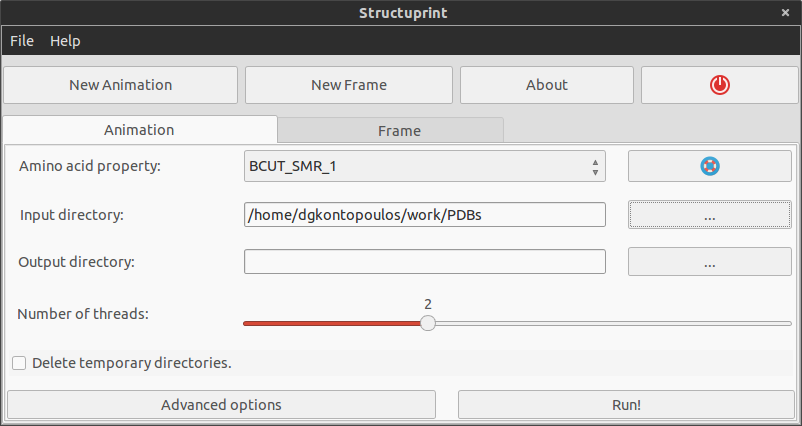
\includegraphics[width=\textwidth]{figures/gui.png}
\end{figure}

The user can switch between two tabs in order to generate an animation or a 
single still image. Some basic options are immediately available, whereas 
all remaining ones can be modified via the 'Advanced options' button.

Clicking 'Run!' launches a temporary terminal in which Structuprint's progress is 
logged. At the end of the run, the user is notified about the status of the 
job (success or failure) and is also prompted to view the resulting figure, if 
successfully generated.

\newpage

\section{Tutorial: visualizing frames from an MD simulation}
Here we will visualize 4 PDB frames from a molecular dynamics 
simulation. We assume that the frames have been superimposed 
to each other prior to this tutorial. The filenames need to have an 
underscore and an ID number before the '.pdb' suffix.
\vspace{-0.5cm}
\begin{figure}[!htbp]
    \centering
	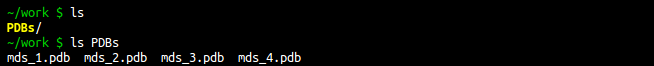
\includegraphics[width=\textwidth]{figures/tutorial/1.png}
\end{figure}

We will then create an empty directory to store Structuprint's output. 
Structuprint will read (\path{-dir}) files from the \path{PDBs} 
directory and save its results (\path{-outdir}) to the \path{Structuprints} 
directory. For coloring, the property it will use (\path{-prop}) is the 
molecular weight one (\path{Weight}). Finally, it will use 4 CPU cores 
simultaneously (\path{-nthreads 4}).
\vspace{-0.5cm}
\begin{figure}[!htbp]
    \centering
	
\includegraphics[width=\textwidth]{figures/tutorial/2.png}
\end{figure}

Running...
\vspace{-0.5cm}
\begin{figure}[!htbp]
    \centering
	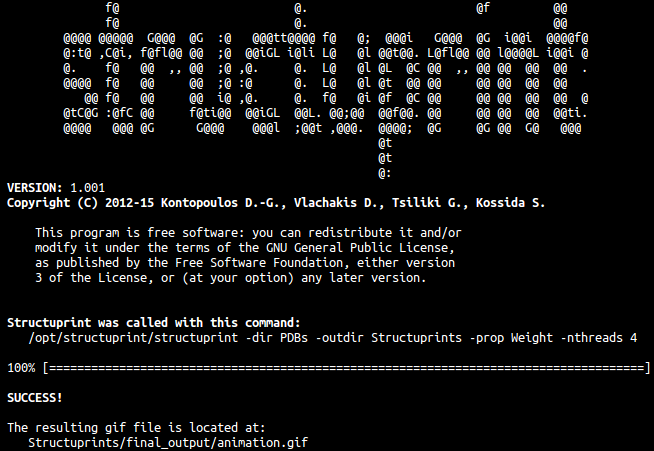
\includegraphics[width=\textwidth]{figures/tutorial/3.png}
\end{figure}

Structuprint created one directory per frame and a \path{final_output} 
directory to store the animation. Each numbered directory contains its 
starting PDB file, a log file and the resulting structuprint figure.
\vspace{-0.5cm}
\begin{figure}[!htbp]
    \centering
	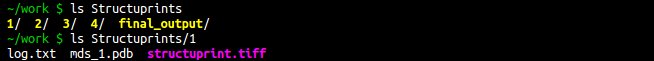
\includegraphics[width=\textwidth]{figures/tutorial/4.png}
\end{figure}

The two-dimensional representations of the PDB structures, as produced 
by Structuprint, are shown below. A simple comparison of the panels 
indicates that a stable conformation has yet to be found.
\vspace{-0.25cm}
\begin{figure}[!htbp]
    \centering
	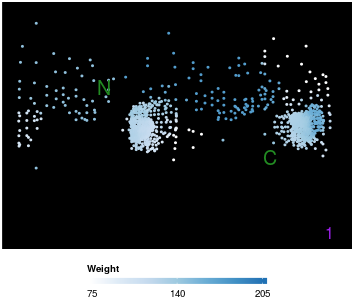
\includegraphics[width=0.45\textwidth]{figures/tutorial/frame_1.png}
	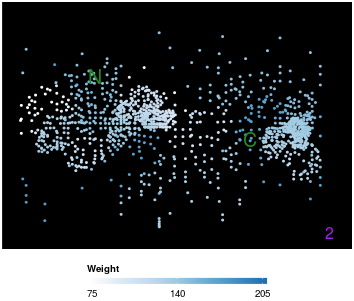
\includegraphics[width=0.45\textwidth]{figures/tutorial/frame_2.png}\\
	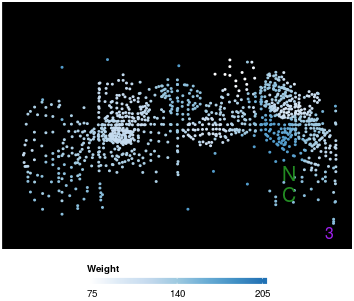
\includegraphics[width=0.45\textwidth]{figures/tutorial/frame_3.png}
	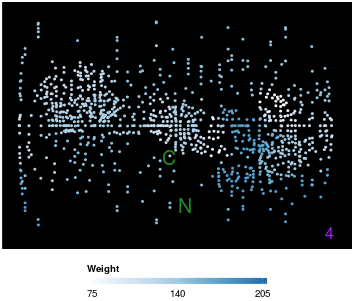
\includegraphics[width=0.45\textwidth]{figures/tutorial/frame_4.png}
	
\end{figure}

\newpage

\section{Common warnings/errors}

\begin{itemize}

\item\textbf{ERROR! No models could be found in that PDB file! Please try and 
fix any format errors. For example, is there an "ENDMDL" keyword after each model?}\\
The number of models is obtained by counting the ENDMDL/END occurrences. You 
can avoid this error by inserting an "END" keyword at the end of the input file.

\item\textbf{Warning! 'XXXX' is not a color that R can understand. 
Setting the background color to '\#000000'.}\\
The \path{-bgcol} parameter allows for changing the background of structuprint 
figures from black to another color. Only HTML hex colors or 
\href{http://www.stat.columbia.edu/~tzheng/files/Rcolor.pdf}{default R colors} 
are supported.

\item \textbf{Warning! A residue (?) for which there is no recorded value was found: HOH\\
Its value was set to 0; that may lead to wrong results!}\\
Structuprint's default database contains values only for the 20 common amino acids. 
If Structuprint detects the presence of a modified amino acid or any other chemical 
component, it will set its value to 0, no matter what property is selected. In 
some rare cases that may not bias the results. For example, if the 
\path{FCharge} property is selected, a ligand with a charge of 0 will not 
affect the final figure, as its value would be set to 0 anyway. In any other 
situation though, the results may be significantly different. The figure below 
shows a structuprint of a PDB file with ligands, with a color scale that 
does not include 0. Grey patches correspond to atoms with a value outside the color 
scale. To fix this issue, see section \ref{sec:extend_db} or \ref{sec:custom_db}.

\begin{figure}[!htbp]
    \centering
	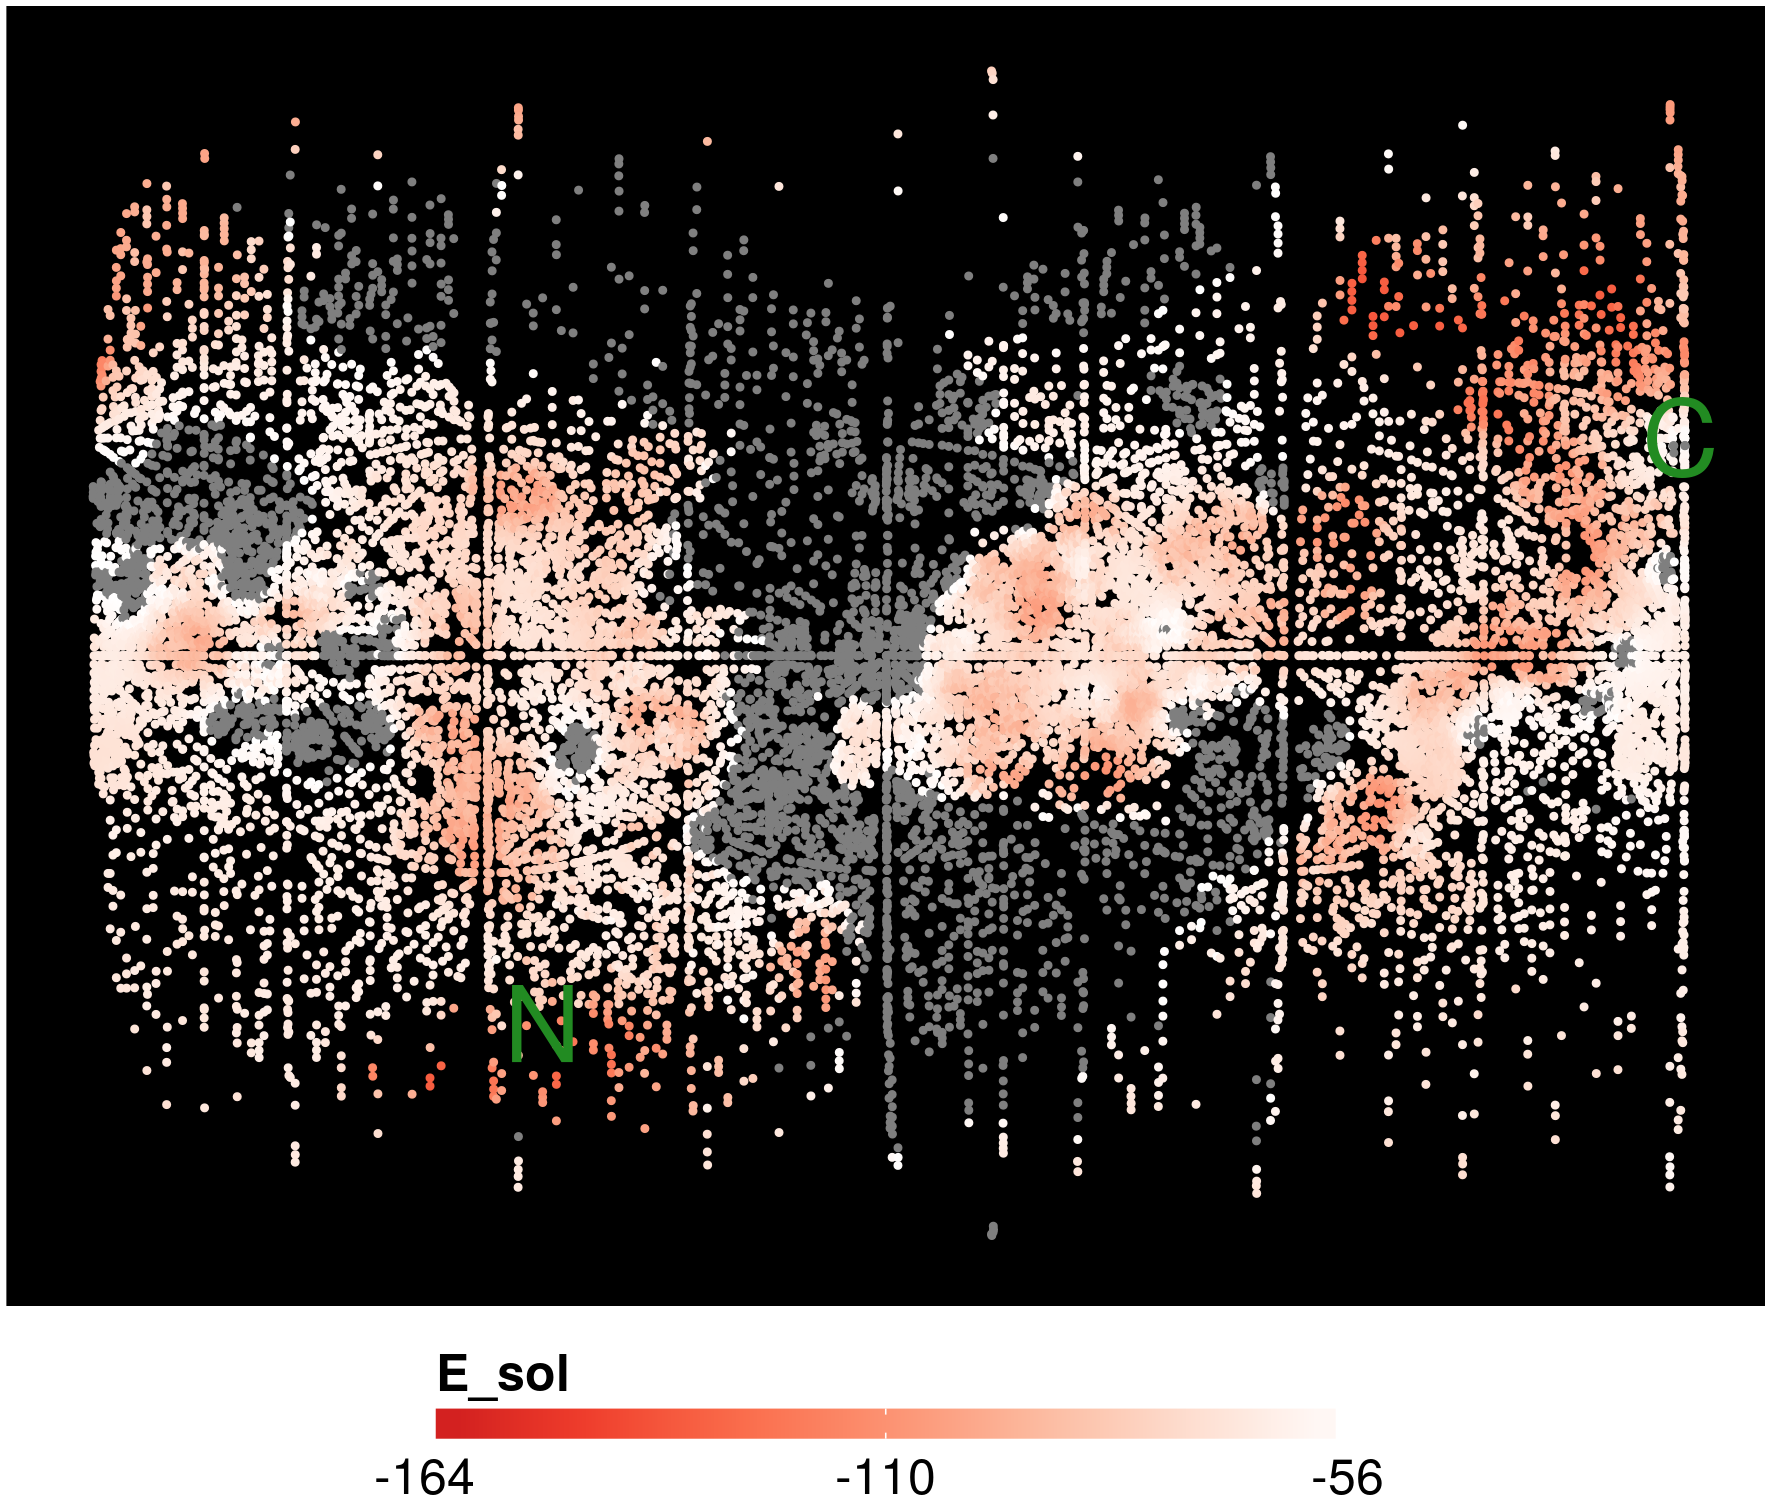
\includegraphics[width=0.7\textwidth]{figures/missing_vals.png}
\end{figure}

\item \textbf{Warning! The width to height ratio (excluding the legend) is not close to 
1.3639. The map will be distorted!}\\
This message appears when both height and width are specified by the user and 
their ratio is not appropriate. The solution would be to enter just the desired 
height or width. Structuprint would then calculate the appropriate value for 
the other dimension.

\end{itemize}

\newpage

\section{Advanced usage}

\subsection{Extending the default database}\label{sec:extend_db}
When faced with a PDB file that contains chemical components for 
which Structuprint does not have measured values, one option is 
to extend the default SQLite database. On GNU/Linux systems, it is usually 
located at \path{/opt/structuprint/amino_acid_properties.db}. 
Each table in the database corresponds to a distinct property and contains 
two columns: i) \path{Amino_Acid} (the 3-letter identifier) and ii) 
\path{Value}.

\begin{figure}[!htbp]
    \centering
	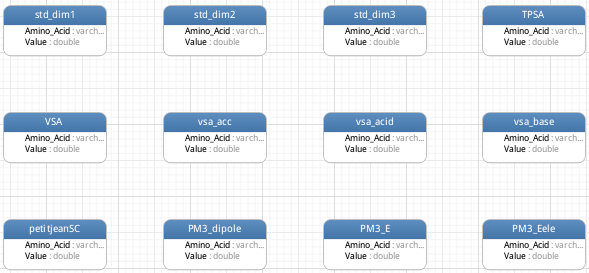
\includegraphics[width=\textwidth]{figures/schema.png}
\end{figure}

To add the molecular weight of a novel chemical component, 
for example, you only have to create a new row in 
the \texttt{weight} table and insert its 3-letter code and its weight 
value.

\subsection{Custom database}\label{sec:custom_db}
A more portable solution would be to create a custom database. 
By doing that, the default database remains in pristine state and new 
properties or measurements are kept in a separate SQLite database. The 
schema should be similar to the one of the default database (see above), i.e. one 
table per property, with columns for the 3-letter code and value. For 
\path{structuprint} or \path{structuprint_frame} to use the custom 
database, you need the \path{-custom_db} option. Note, however, that 
\textbf{Structuprint will only read values from one database at a time} and will 
not combine measurements from both databases!\\

\begin{myboxii}[\begin{center}Resources for properties of chemical components\end{center}]
\begin{tabular}{ll}
-PDBeChem: & \url{https://www.ebi.ac.uk/pdbe-srv/pdbechem/}\\
-PubChem: & \url{http://pubchem.ncbi.nlm.nih.gov/}\\
-DrugBank: & \url{http://www.drugbank.ca/}\\
-ChemSpider: & \url{http://www.chemspider.com/}\\
\end{tabular}
\end{myboxii}

\newpage
\section{Known issues}
\begin{itemize}
\item \textbf{When the dimensions of the structuprint are small, data points may overlap.} 
This usually leads to some degree of color variation even betwen different runs against the 
same PDB file, as the data points are drawn in random order. To address that issue, 
you could reduce the size of the data points by setting \path{-point_size} to 
a value that is smaller than 1. Alternatively, increasing the size of the figure 
will provide enough space for overlapping not to occur.\\

\item \textbf{When the ID number is plotted on the structuprint, there may be 
some small differences in the color scale between frames (see below).} The colors 
preserve their positions across the scale, but the borders between them may 
slightly fluctuate. This problem does not occur when the ID number is omitted 
from the figure (\path{--no_ID}) and is possibly a shortcoming of the 
underlying \path{ggplot2} R code that Structuprint uses.
\vspace{-0.25cm}
\begin{figure}[!htbp]
    \centering
	
\includegraphics[width=\textwidth]{figures/legend_diffs.png}
\end{figure}

\end{itemize}
\end{document}
